\documentclass[a4paper,10pt]{article}

% Hier die Nummer des Blatts und Autoren angeben.
\newcommand{\blatt}{9}
\newcommand{\autor}{Merlin Steuer, Till Schander, Lennart Bergmann}

\usepackage{hci}

\begin{document}
% Seitenkopf mit Informationen
\kopf
\renewcommand{\figurename}{Figure}

\aufgabe{14}
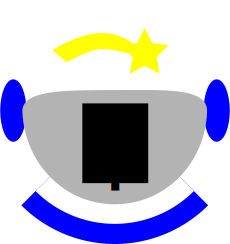
\includegraphics[scale=0.6]{Icon.png}

Das Icon soll für eine App sein, welche es Astronauten ermöglich, mithilfe einer Weltraumfähigen Smartwatch oder ähnlichen im Raumanzug verbauten Gerätschaften einen solchen zu überwachen. Es soll eine Möglichkeit geben, aktuelle Parameter des Anzugs wie bspw. Sauerstoffvorat, Temperatur u.s.w. auszulesen, als auch die derzeitigen Vitalparameter des Trägers (Puls, Blutdruck, Atemfrequenz) zu beobachten.

Es stellt einen stilisierten Helm eines Raumanzuges dar. Das Blau wurde gewählt, da dies die Farbe des Himmels bzw. des Weltraums ist - ungeachtet der Tatsache, dass die Aussicht des Astronauten selbst aus deutlich dunkleren Tönen besteht. Das Kreissegment am unteren Rand stellt den Kragen bzw. Halsansatz des Trägers dar, um zu verdeutlichen, dass es sich um einen Helm handelt. Das Visier ist grau, um sich vom Rest des Helms abzusetzen. Übliche reelle Visierfarben wie Silber oder Gold (wegen der besseren Reflektion von Licht bzw. Energie/Wärme) wären hier zu dominant.

Da der Helm eine hohe Ähnlichkeit zu Taucherhelmem besitzt, wurde ein angedeuteter Stern mit Schweif angefügt, um Missverständnisse zwischen Astronauten und Berufstauchern (für welche eine ähnliche App sicher denkbar und sinnvoll wäre) zu vermeiden. Um die Strukturen des Bildes nicht zu komplex werden zu lassen, wurde ein einfacher, 5-Zackiger Stern gewählt mit einem simplen gebogenen Schweif. Gelb war die offensichtlichste Farbe, welche sich auch gut vom Hintergrund abhebt.

Da es sich zunächst um eine rein informative App handelt, welche keine Möglichkeit bietet, Manipulationen am Raumanzug vorzunehmen, ist noch das typische Informations-i ins Visier eingepasst worden. Somit hat der Benutzer in seinem im Arm eingearbeiteten Display direkt den Überblick, was die App leistet.

Es wurde versucht, bei der Platzierung und Dimensionierung der Elemente des Icon den goldenen Schnitt einzuhalten (Visier:Helm, Größe/Position des i, Gestaltung der Sternschnuppe), gelungen ist dies leider mäßig.
\end{document}
